\documentclass{article}

% If you're new to LaTeX, here's some short tutorials:
% https://www.overleaf.com/learn/latex/Learn_LaTeX_in_30_minutes
% https://en.wikibooks.org/wiki/LaTeX/Basics

% Formatting
\usepackage[utf8]{inputenc}
\usepackage[margin=1in]{geometry}
\usepackage[titletoc,title]{appendix}

% Math
% https://www.overleaf.com/learn/latex/Mathematical_expressions
% https://en.wikibooks.org/wiki/LaTeX/Mathematics
\usepackage{amsmath,amsfonts,amssymb,mathtools}

% Images
% https://www.overleaf.com/learn/latex/Inserting_Images
% https://en.wikibooks.org/wiki/LaTeX/Floats,_Figures_and_Captions
\usepackage{graphicx,float}

% Tables
% https://www.overleaf.com/learn/latex/Tables
% https://en.wikibooks.org/wiki/LaTeX/Tables

% Algorithms
% https://www.overleaf.com/learn/latex/algorithms
% https://en.wikibooks.org/wiki/LaTeX/Algorithms
\usepackage[ruled,vlined]{algorithm2e}
\usepackage{algorithmic}

% Code syntax highlighting
% https://www.overleaf.com/learn/latex/Code_Highlighting_with_minted
\usepackage{listings}
%\usepackage{minted}
%\usemintedstyle{borland}

\usepackage{hyperref}
\usepackage{subcaption}
\usepackage{bm}

% References
% https://www.overleaf.com/learn/latex/Bibliography_management_in_LaTeX
% https://en.wikibooks.org/wiki/LaTeX/Bibliography_Management
%\usepackage{biblatex}
%\addbibresource{references.bib}

% Title content
\title{AMATH 582 Homework Five: Background Subtraction}
\author{Daniel W. Crews}
\date{March 10, 2021}

\begin{document}

\maketitle

% Abstract
\begin{abstract}
  The dynamic mode decomposition (DMD) analyzes data into spatiotemporally-correlated modes of varying complex frequencies. This work looks at a simple example of the DMD by solving the problem of video background separation. This is accomplished by subtracting the lowest frequency modes from a video clip, with the wrinkle of negative pixel values dealt with in video-dependent ways. Generally negative values can simply be subtracted out. Yet in a video of a skiier, the snow is much brighter than the skiier so subtracting out negative values removes the skiier too. For this clip, the negative pixels are flipped to their absolute values. %he DMD has many other significant uses such as in linear control theory.
  %Measurements generically include superfluous components (from the perspective of an analyst at least). An old, efficient, and quite spectacular method to extract particular dynamics within a dataset is called principal component analysis (PCA). Basically, PCA is an eigendecomposition of the covariance matrix. This report utilizes PCA to analyze simple harmonic motion recorded on separate video cameras, assigning different oscillatory components to particular modal coordinates rather their motional ones. %rather than dispersed between various different ones. % Spectral analysis consists of far more than determination of the Fourier coefficients of a time series. This numerical experiment explores the spatial distribution of a signal's frequency spectrum (or spectrogram) through the pratical examples of classic shredding moments in music history (here, Guns and Roses and Pink Floyd). To compute the spectrograms a short-time (masked) Fourier transform is used, and in particular this report explores its filtering using the Wigner distribution function of the time series. Here the Wigner function is computed as an $\mathcal{O}(N^2)$ operation in terms of the Fourier coefficients.
    %Signal processing is used ubiquitously in science and engineering. This simple numerical experiment explores an important aspect of signal analysis, namely statistical averaging of a spectral time series to eliminate noise and thereby identify center frequencies. Here the time series consists of a spatial wavefield which is denoised via Gaussian filtering about the identified frequency to determine a trajectory. While the technique explored in this report is quite elementary compared to more sophisticated signal processing approaches, it conveys the essential elements of, for example, a radar or sonar tracking system. %In this case such a trajectory is determined from a noisy waveform in a time series of three spatial dimensions. 
\end{abstract}

% Introduction and Overview
\section{Introduction and Overview}
This work separates the background from two short video clips, one of race cars and the other of a skiier. This is done using the dynamic mode decomposition (DMD) method, which approximates the Koopman operator that evolves the video as a dynamical system. Importantly, both images have little camera wobble, so the singular value decomposition (SVD) is able to identify orthogonal modes of spatiotemporal correlation and isolate the background. The DMD then approximates the Koopman operator on these modes according to a multistep process outlined in Section \ref{theory}. Having singled out the lowest frequency modes for a pure background reconstruction, this is then subtracted from the video clips to accomplish background separation.

% The first section of this report briefly summarizes the SVD theory and that of the linear classifiers, before proceeding into the results of analysis in the second section. Here the various classification methods are compared to one another, in particular on difficult-to-distinguish digit pairs. However, here it's found that the SVM method sorts these with good accuracy. While this analysis utilized the entire training and test dataset and hence had a deterministic outcome, in practical application of these methods cross-validation (repeated classification with a randomly sampled training dataset) is needed to demonstrate robustness.
%Here four expriments are analyzed of videos taken from three perspectives of a mass oscillating at the end of a string. The four experiments consisted of simple one-dimensional harmonic motion in gravity from the string tension, then introduction of an additional swinging pendulum motion, and thirdly also rotation of the oscillating mass. Finally data was collected with camera shake in order to introduce measurement noise. The measurements are composed of multiple relatively independent simultaneously occuring oscillations to demonstrate the mathemagical properties of the principal component analysis (PCA) method, which separates oscillatory modes by an eigendecomposition (thus, diagonalization) of the data covariance matrix.

%The purpose of this work is to visualize some of the most famous shredding in rock and roll history (Pink Floyd and Guns and Roses (GNR)) by construction of a spectrogram. Section \ref{theory} outlines the theory of the combined Gabor-Wigner distribution used for the spectrogram, followed by a section detailing implementation of the algorithm. Results are presented for the opening guitar riff in GNR, bass line in Floyd, and a stab at the Floyd guitar solo. The attached appendices describing elements of Wigner distributions are hoped not to count towards the overall page limit and included merely for completeness. The report itself is kept concise.

% This report describes an algorithm used to denoise the signal via a statistical method and to identify the submarine's trajectory. It begins with a brief theoretical overview of the methods used, and proceeds to a discussion of the details of the code used to implement the methods. There is then a discussion of results identifying the three-dimensional trajectory, along with a suggested search area for a submarine-tracking aircraft and the likely frequency of the submarine. The report is kept brief without sacrificing clarity.

% Theoretical Background
\section{Theoretical Background}\label{theory}
\subsection{Dynamic mode decomposition}
In this class, previous works studied the decomposition of a data matrix into its proper modes using the SVD operation. These frames, such as handwriting examples, were not time-dependent. Yet in a video clip (or time series data) each realization is separated from its neighbors by a time difference $\Delta t$. If the video is collected into an array $X\in\mathbb{R}^{n\times m}$ of dimension (pixels$\times$time), and a second array $X'$ is formed one difference $\Delta t$ into the future, then the two may be supposed to be related by a Koopman evolution operator,
\begin{equation}
  X' = AX
\end{equation}
where $A$ is taken to solve the problem in the least-squares Moore-Penrose pseudoinverse $Y^+$ sense \cite{kutz}. However, this makes $A = X'X^+$ a (pixels$\times$pixels) operator. Generally speaking this matrix $A$ will be too large to perform an eigenvalue decomposition on directly with any efficiency. On the other hand, dynamic mode decomposition tackles this problem by projecting into a low-rank truncation of $X$ obtained via SVD,
\begin{equation}
  X_r = U_r\Sigma_rV_r^\dagger
\end{equation}
with $r$ the truncation order. Therefore the Koopman operator $A$ may be represented in this subspace,
\begin{equation}
  \widetilde{A} \equiv U_r^\dagger A_rU_r = U^\dagger X'V_r\Sigma_r^{-1}
\end{equation}
with $\widetilde{A}\in\mathbb{C}^{r\times r}$. Having identified an approximate $A$, a more tractable eigendecomposition is performed
\begin{equation}
  \widetilde{A}W = W\Lambda.\label{eigs}
\end{equation}
The orthogonal modes of the low-dimensional evolution operator are then lifted to the full-rank space by
\begin{equation}
  \Phi \equiv X'V_r\Sigma_r^{-1}W
\end{equation}
and the fundamental frequencies computed via $\Omega \equiv \log(\Lambda)/\Delta t$. By this method the DMD has been accomplished according to the approximate continuous-time reconstruction
\begin{equation}
  \widetilde{X}(t) = \Phi\exp(\Omega t)b
\end{equation}
where $b$ is the vector of initial conditions obtained via $b = \Phi^+X(0)$. This reconstruction is approximate in the sense that high mode dynamics have been disregarded \cite{kutz_dmd}.

\subsection{Background subtraction method}\label{background}
The above is the standard DMD method. In this work, a slight variation is used to perform the background subtraction. By examination of the eigenvalue spectrum $\Lambda$ of the low-dimensional operator of Eqn. \ref{eigs}, the lowest frequency modes $\Lambda_L$ (usually just one or two) are extracted and its reduced eigenvector $W_L$ used to construct the low-frequency DMD operator $\Phi_L$ \cite{kutz_dmd}. The method then proceeds as normal. A slight variation on the method presented in Ref. \cite{kutz_dmd} is used, wherein the best-fit background $b(t)$ is identified for each time increment by calculating $b(t_i) = X(t_i)\Phi^+$ rather than exponentially evolving the frequencies. This was found to work better, but they are perhaps equivalent and the author may simply have had a bug.

% Algorithm Implementation and Development
\section{Algorithm Implementation and Development}\label{section}
Each video consists of a number of frames at sixty frames-per-second. These are loaded in, converted to grayscale, and then analyzed by the DMD algorithm of Section \ref{theory}. For each video the low-rank truncation of $X_r$ used to construct $\widetilde{A}$ was chosen to be 100 modes. The resulting eigenvalue spectrum of of $\widetilde{A}$ is shown in Fig. \ref{eigs_pics_mc} and \ref{eigs_pics_sd} for the race cars and skiier respectively. It was found that four race car modes and five skiier ones were sufficient for background reconstruction. Experimentation on the precise number of low-frequency modes was found not to be significant provided that there were enough of them, \textit{but} not too many.

\begin{figure}[b!]
  \centering
  \includegraphics[width=0.45\textwidth]{montecarlo_dmd_spectrum}\quad\quad\quad\includegraphics[width=0.45\textwidth]{montecarlo_low_spectrum}
  \caption{Spectrum of the low-rank approximate race car Koopman operator $\widetilde{A}$ using an $r=100$ truncation. Evidently the the low-frequency activity is clustered around a cloud of modes. The four lowest modes were found to provide a good low-frequency reconstruction according to the method of Section \ref{background}.}\label{eigs_pics_mc}
\end{figure}

\begin{figure}[t!]
  \centering
  \includegraphics[width=0.45\textwidth]{skidrop_dmd_spectrum}\quad\quad\quad\includegraphics[width=0.45\textwidth]{skidrop_low_freq_spectrum}
  \caption{Eigenvalues of the skiier video operator approximated with one hundred modes. Here, the sparse background is observed to occupy mostly one mode, with a far sparser low-frequency spectrum than the race car video. The five smallest modes are used to account for slight variations and background wobble.}\label{eigs_pics_sd}
\end{figure}

According to the identified eigenvalues, the background was then reconstructed using $X_L(t_i) = \Phi_L b(t_i)$ with each coefficient $b(t_i) = \Phi_L^+X(t_i)$ found via pseudoinverse. As $X_L$ is complex, one then subtracts the background using the element-wise absolute value of the low-frequency modes per timestep
\begin{equation}
  X_S(t_i) = X(t_i) - |X_L(t_i)|.\label{sparse}
\end{equation}

\section{Computational Results}
With the reconstructed backgrounds (seen at $t=0$ in Fig. \ref{backgrounds}) the $X_S(t_i)$ were calculated for each video. Different methods were then used to deal with the resulting negative values in the sparse reconstruction $X_S$. For example, in the skiier video the person skiing is dark compared to the bright snow, so the skiier pixels in Eqn. \ref{sparse} are very negative. Then to really pull out the skiier against the mostly-zero subtracted field, the absolute value of the pixels are taken and the result plotted on a $[0,255]$ grayscale. A still is seen in Fig. \ref{skiiers}.

In contrast, the race car video had more camera drift so that the background reconstruction was not perfect every time. The difference was typically negative, so adding these back in via the method described in the assignment (\textit{i.e.} setting them to zero) and was found to work better than the above approach for the skiier video. This is shown in Fig. \ref{montecarlo}. However, the background subtracted video $|X_S|$ still more clearly contained the race cars. Here there were other artifacts, such as the yellow road marker appearing on top of the reconstructed cars. A sample of these more clearly visible cars with other artifacts is shown in Fig. \ref{montecarlo2}.

\begin{figure}[hb!]
  \centering
  \includegraphics[width=0.45\textwidth]{skiier_color}\quad\quad\quad\includegraphics[width=0.455\textwidth]{skiier}
  \caption{The skiier against a beautiful mountain scene (left) and with the background subtracted (right).}\label{skiiers}
\end{figure}

\begin{figure}[ht!]
  \centering
  \includegraphics[width=0.45\textwidth]{racecars3}\quad\quad\quad\includegraphics[width=0.455\textwidth]{racecars3_nbg}
  \caption{Race cars in a fancy European city (left) and without their background (right).}\label{montecarlo}
\end{figure}

% \begin{figure}[hb!]
%   \centering
%   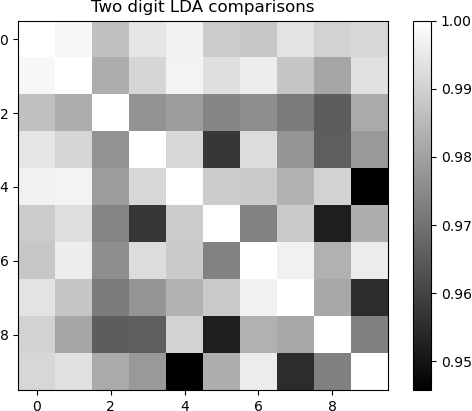
\includegraphics[width=0.4\textwidth]{2dgt_error_lda_50modes}\quad\quad\quad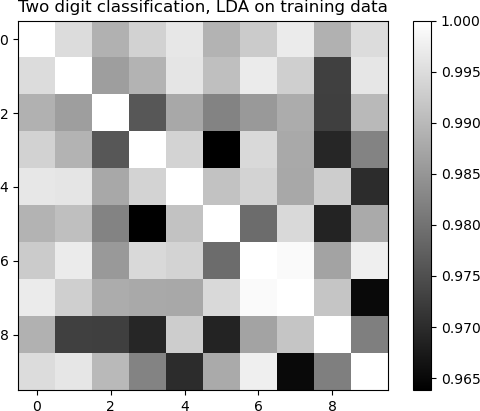
\includegraphics[width=0.4\textwidth]{ontrainingdata/lda_allmodes}
%   \caption{Classification score of LDA method on digit pairs. (Left:) scores of the test data using 50-mode reduced training data. While all scores are $>94$\%, 2 has a poor trend and certain pairings are not good.\\(Right:) Classifier score on its own training data without dimension reduction, showing inherent LDA error.}\label{lda}
% \end{figure}

% \begin{figure}[ht!]
%   \centering
%   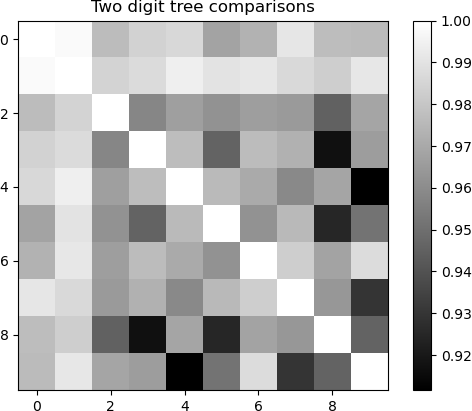
\includegraphics[width=0.4\textwidth]{2dgt_tree_50modes}\quad\quad\quad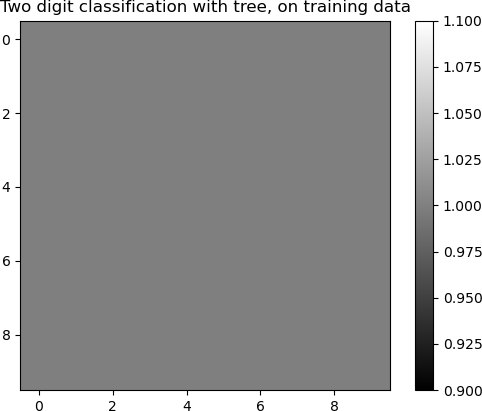
\includegraphics[width=0.4\textwidth]{ontrainingdata/tree_training}
%   \caption{(Left:) Two-digit classification results using the decision tree method. Interestingly, larger errors are observed compared to the LDA, but the digit 2 consistently performs better. Errors on the difficult-to-distinguish pairs of the LDA are exacerbated by the decision tree. (Right:) The tree, at least with default settings, predicts its own training data exactly (so the colorbar was autoset). This indicates overfitting.}\label{tree}
% \end{figure}

% Further, predicting the original training data reveals the very same error pattern, though at a lower rate of incidence. This demonstrates an inherent error in the LDA method due to outliers, even though it operates on a minimized Rayleigh quotient. Now Fig. \ref{tree} demonstrates results with the decision tree method. The main takeaway from these results is that errors on difficult-to-distinguish data are made even worse by the decision tree compared to the LDA, but it predicts its own training data very well.

% Next, the support vector machine was explored with results in Fig. \ref{svm}. The SVM was observed to be calculated faster than the decision tree \textit{and} to have accurate results to within almost 1\%! However, it has a small rate of error in predicting its own training data. As before, the SVM was trained on a 50-mode reduced dimension eigenprojected dataset. Comparison of Figs. \ref{lda}, \ref{tree}, and \ref{svm} shows that all three methods distinguish 0 and 1 very well, and all have the most difficulty with 4 and 9. However, the SVM classifier predicts with great accuracy and beats the others by several percentage points.

% It must be stressed that this analysis is done deterministically on a single set of training and test data. Generally speaking these methods are to be cross-validated by randomly sampling a subset of the training data and doing a statistical analysis of the resulting scores for different training set sizes. The author played around with this a bit while doing the assignment but did not include these results for brevity. The general trend was that scores were lower when using a smaller training set, but the SVM still did the best.

% \begin{figure}[hb!]
%   \centering
%   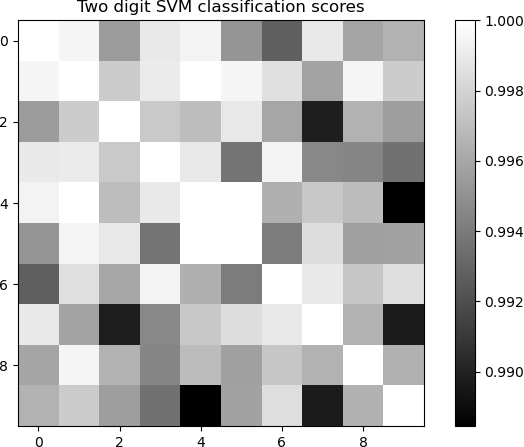
\includegraphics[width=0.4\textwidth]{2dgt_svm_50modes}\quad\quad\quad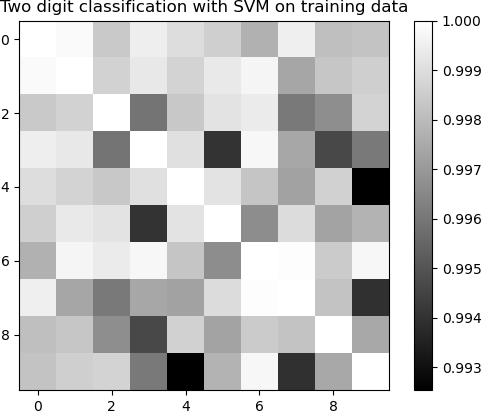
\includegraphics[width=0.4\textwidth]{ontrainingdata/svm_training}
%   \caption{Two-digit classification results with the SVM method. The support vector technique is seen to be the best of the three methods overall, and intriguingly has almost perfect discernment between digits 4 and 5. It stumbles most on 4 and 9, however perhaps even a human would on these digits when handwritten.}\label{svm}
% \end{figure}

% \begin{figure}[ht!]
%   \centering
%   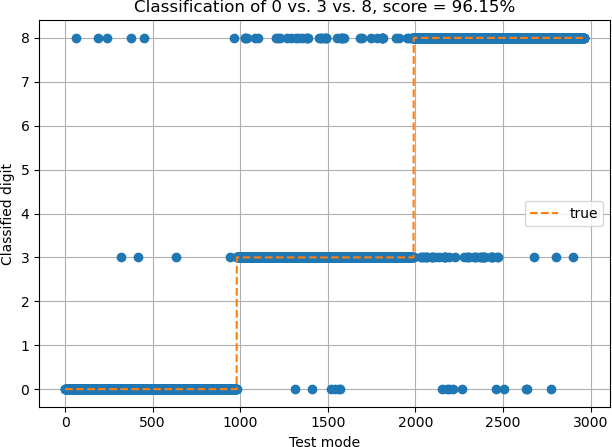
\includegraphics[width=0.315\textwidth]{lda3/3digit_lda_038}\quad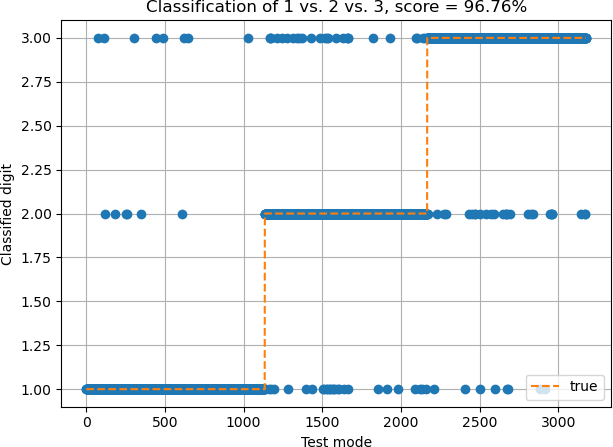
\includegraphics[width=0.315\textwidth]{lda3/3digit_lda_123}\quad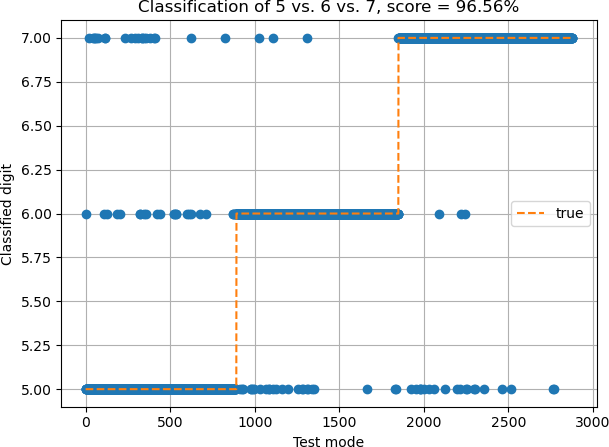
\includegraphics[width=0.315\textwidth]{lda3/3digit_lda_567}
%   \caption{Simultaneous classification of three digits using LDA on the sets of digits 038, 123, and 567. Generally good classification in line with the ``worst'' results of the two-digit LDA is observed, here $> 96$\%.}\label{threedigit}
% \end{figure}

% \subsection{Three-digit classification}
% As an initial exploration of further capabilities, Fig. \ref{threedigit} shows LDA applied to categorize three digits simultaneously. Good results are seen in these cases, with general trends in line with the results of the two-digit LDA in Fig. \ref{lda}. However, one would expect that simultaneous classification of all nine digits would run into issues due to the general mixing of eigenvalues for the difficult pairs such as 9 and 4, contaminating performance of the entire classification scheme. Three digits was generally seen to work well though.

% \begin{figure}[h]
%   \centering
%   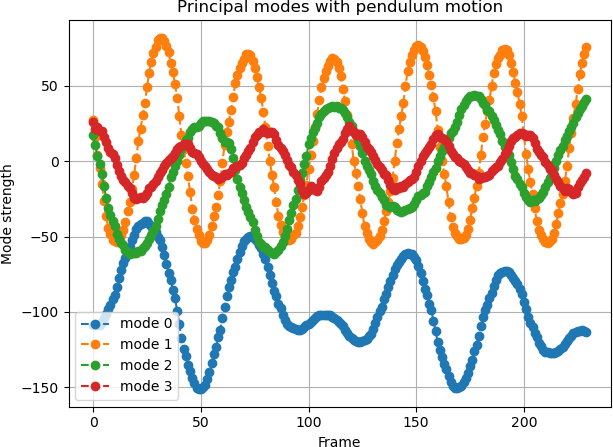
\includegraphics[width=0.45\textwidth]{pca_pend2}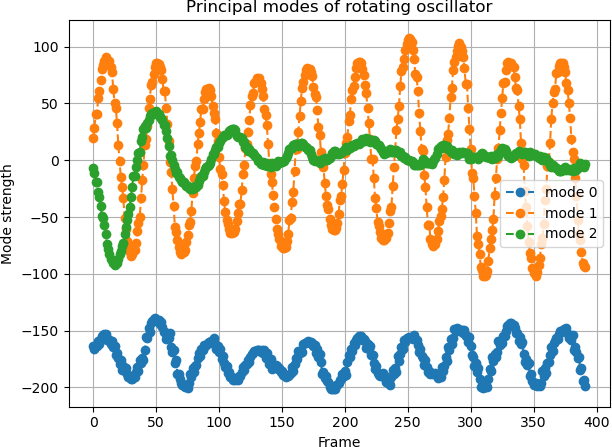
\includegraphics[width=0.45\textwidth]{pca_rotate2}
%   \caption{Projected modes of bucket coordinates for cases of SHM superimposed on pendulum motion (left) and bucket rotation (right). In comparison to the baseline case (Fig. \ref{sns}) clearly ``mode 1'' still describes the bucket SHM as their frequencies match. The pendulum motion appears as a lower-frequency oscillation apparently in ``mode 2''. However, the occurence of both oscillations appears to leave a modulated trace (superposition?) in mode 0, in curious correlation with the Wigner function experiments of the last homework. The rotating oscillator case shows a damped rotation tendency in ``mode 2,'' matching the video here.}\label{pr}
% \end{figure}

% \begin{figure}[hb!]
%   \centering
%   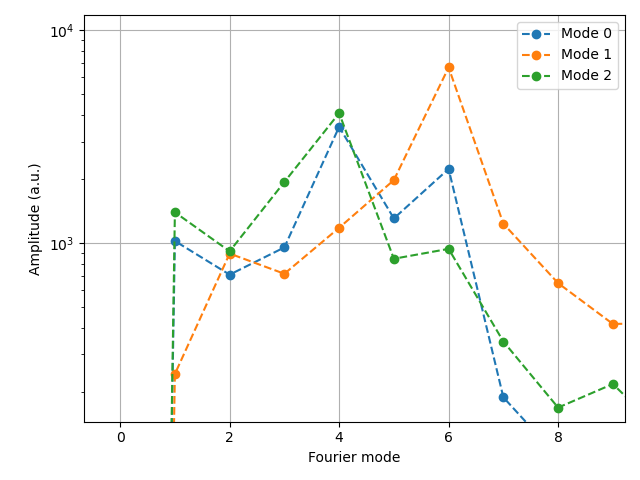
\includegraphics[width=0.5\textwidth]{pendulum_fft3}
%   \caption{First few Fourier components from FFT of the pendulum case, showing the frequencies in the ``mode 0'' waveform to be the SHM and pendulum frequencies 4 and 6, and perhaps interference in mode 5.}\label{pend_fft}
% \end{figure}

% \begin{table}[b]
%   \centering
%   \begin{tabular}{|l|l|l|l|l|l|l|l|l|}
%     \hline
%     Time {[}hr{]}   & 0-3.5 & 3.5-7.0 & 7.0-10.5 & 10.5-14.0 & 14.0-17.5 & 17.5-21.0 & 21.0-24.5 & All-time average \\ \hline
%     $\langle k_x\rangle_T$ {[}1/L{]} & 0.814 & 0.661   & 0.784    & 0.760     & 0.810     & 0.728     & 0.802     & 0.766            \\ \hline
%     $\langle k_y\rangle_T$ {[}1/L{]} & 0.271 & 0.292   & 0.331    & 0.240     & 0.341     & 0.267     & 0.271     & 0.288            \\ \hline
%     $\langle k_z\rangle_T$ {[}1/L{]} & -1.00 & -1.03   & -1.09    & -1.06     & -1.13     & -1.07     & -1.1125   & -1.07            \\ \hline
%   \end{tabular}
%   \caption{Observed center frequencies of data following spectral averaging over time intervals of $3.5$ hours, with seven samples per interval, then used as the filter frequencies $k_0$ in the Gaussian filter. The arbitrary spatial unit is given as $L$, not to be confused with domain length. The all-time average is given as well.}\label{frequencies}
% \end{table}

% Note that in Table \ref{frequencies} negative wavenumbers are used as the given spatial data is complex, meaning that the reality condition is not satisfied, instead $\hat{f}(-k) = \hat{f}^*(k)$ in this dataset. The absolute value is reported as ``the frequency'' of the submarine, however. This identifies the submarine's spectral signature as $\bm{k} \approx \{0.766 \pm 0.05, 0.288 \pm 0.03, 1.07 \pm 0.04 \}$ {[}1/L{]} by mean and standard deviation of the window averages of Table \ref{frequencies}, where L is an arbitrary space unit corresponding to that of the provided data, \textit{not} the domain length. The width of the space or frequency ``submarine Gaussian'' was not measured for ease of analysis.

% Having computed the center frequencies, the spectrum was filtered and the trajectory determined according to the schematic Steps 4 and 5. The resulting 3D trajectory and top-down position given in Figs. \ref{traj:3d}, \ref{traj:2d} respectively. This suggests the submarine is currently located around $\bm{x}\sim(-5, 6.5)$ in $(x,y)$.

% \begin{figure}[hb]
%   \centering
%   \begin{subfigure}{0.42\textwidth}
%     \centering
%     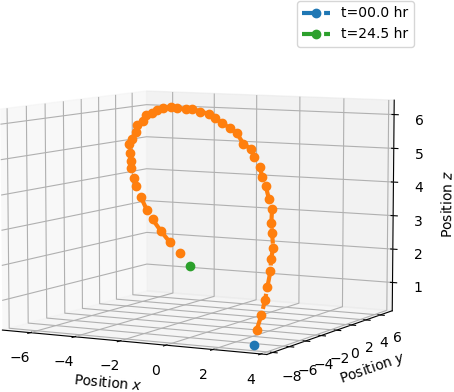
\includegraphics[width=0.99\linewidth]{pics/3d_traj}
%     \caption{Three-dimensional trajectory of submarine, showing a rise and dive maneuver.}\label{traj:3d}
%   \end{subfigure}
%   \begin{subfigure}{0.42\textwidth}
%     \centering
%     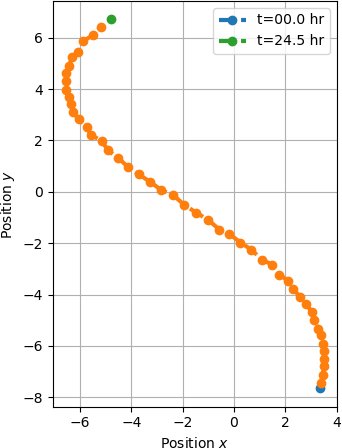
\includegraphics[width=0.6\linewidth]{pics/2d_traj}
%     \caption{Top-down view of predicted trajectory. Ideal search area for submarine-tracking aircraft is around $\bm{x} \sim (-5, 6.5)$ and continuing north-east.}\label{traj:2d}
%   \end{subfigure}
%   \caption{Identified submarine trajectory sampled 49 times in a 24.5 hour period, in 3D and 2D projections.}
% \end{figure}

% Summary and Conclusions
\section{Summary and Conclusions}
This numerical experiment looked at the very versatile and downright amazing dynamic mode decomposition (DMD) method, which can identify the temporal behavior of spatiotemporally-correlated modes identified by the SVD. This is effectively an approximation to the Koopman operator describing the possibly infinite-dimensional linear evolution of some difficult-to-describe nonlinear dynamics. While this Koopman operator can in principle be directly approximated using the pseudoinverse of a single time differenced data matrix $X'$, the resulting matrix $A$ is generally far too large for eigendecomposition. The DMD first projects into a low-rank subspace containing the most important modes, as seen by the largest singular values of the data matrix $X$. A low-dimensional Koopman operator is then eigendecomposed and lifted back into the full data space using the SVD basis operators. While not orthogonal, these modes are in a sense the best ones to represent the general dynamics of the data.

The biggest advantage of the DMD is that it provides a linear time-dependent representation of the dynamics behind data. This work used the lowest frequency modes for a simple example of the DMD's utility, namely in image background separation. However, there is far more potential in the DMD than this application. By obtaining a linear representation for system dynamics control theory can be applied for a great variety of engineering tasks. Most of these control applications involve something akin to the inverted pendulum problem; that is, sufficient data collection, DMD processing, and control may be used to stabilize generally unstable nonlinear systems such as magnetic confinement systems. Thank you all for teaching this! Code and background-subtracted videos are available on the author's Github \href{https://github.com/crewsdw/amath582}{here}.

\begin{figure}[b!]
  \centering
  \includegraphics[width=0.425\textwidth]{racecars_av}
  \caption{The absolute value of the sparse reconstruction $|X_S(t)|$ gave better image quality than Fig. \ref{montecarlo2} yet with more artifacts such as the street appearing on top of the car, seen here on the left side of the first car.}\label{montecarlo2}
\end{figure}

% % References
\bibliographystyle{unsrt}
\bibliography{references}

\begin{figure}[t!]
  \centering
  \includegraphics[width=0.65\textwidth]{montecarlo_background}\quad\includegraphics[width=0.3\textwidth]{skidrop_background2}
  \caption{Background reconstructions of race cars (left) and skiier (right) using the low-frequency modes.}\label{backgrounds}
\end{figure}

% % Appendices
\begin{appendices}

% \newpage
% % MATLAB Functions
\section{Python Functions}\label{functions}
The following list compiles important Python functions used in implementation:
\begin{itemize}
\item The commands \texttt{np.linalg.svd(X)} and \texttt{np.linalg.eig(X)} are used for big linear algebra operations,
\item The \texttt{av} package was used to read in the \texttt{.mp4} video clips,
\item The sequence \texttt{np.argsort(np.abs(freqs))} sorts the eigenvalues by their absolute value.
\end{itemize}

% % MATLAB Codes
\section{Python Implementation}\label{implementation}
% A separate analysis script was used for each dataset and the files are quite similar. Only pendulum is shown for brevity (see Github page for other files).
% % Wigner function file \texttt{fourier.py}:
% \lstinputlisting{wpendulum.py}
% \vspace{5cm}
Main implementation file \texttt{hw5.py}:
\lstinputlisting{hw5.py}
% \begin{listing}[h]
% \inputminted{matlab}{example.m}
% \caption{Example code from external file.}
% \label{listing:examplecode}
% \end{listing}

\end{appendices}

\end{document}